% THIS IS AN EXAMPLE DOCUMENT FOR VLDB 2012
% based on ACM SIGPROC-SP.TEX VERSION 2.7
% Modified by  Gerald Weber <gerald@cs.auckland.ac.nz>
% Removed the requirement to include *bbl file in here. (AhmetSacan, Sep2012)
% Fixed the equation on page 3 to prevent line overflow. (AhmetSacan, Sep2012)

\documentclass{vldb}
\usepackage{graphicx}
\usepackage{balance}
\usepackage{url}
\usepackage{times,amsmath,epsfig}
\usepackage{graphicx}
\usepackage{amsfonts}
\usepackage{algorithm} 
\usepackage{algorithmic}  
\usepackage[algo2e,linesnumbered]{algorithm2e} 
\usepackage{amsfonts}
\usepackage{amsbsy}
\usepackage{graphicx}
\usepackage{physics}
\usepackage{color}
\usepackage{subfigure}
\usepackage{booktabs}
\usepackage{multirow}
\usepackage{paralist}
\graphicspath{ {images/} }
\setlength{\tabcolsep}{2pt}
% \setlength{\textfloatsep}{9pt}

\newcommand{\cs}[1]{\texttt{\char`\\#1}}
\newcommand{\X}{\mathcal{X}}
\newcommand{\f}{\mathbf{f}}
\newcommand{\Y}{\mathcal{Y}}
\newcommand{\F}{\mathcal{F}}
\newcommand{\Set}{\mathcal{S}}
\newcommand{\Loss}{\mathcal{L}}
\newcommand{\R}{\mathcal{R}}
\newcommand{\K}{\mathfrak{K}}
\newcommand{\x}{\mathrm{x}}
\newcommand*\Bell{\ensuremath{\boldsymbol\ell}}


% Include information below and uncomment for camera ready
\vldbTitle{Data Synthesis based on Generative Adversarial Networks}
\vldbAuthors{Noseong Park, Mahmoud Mohammadi, Kshitij Gorde, Sushil Jajodia}
\vldbDOI{https://doi.org/TBD}

\begin{document}

% ****************** TITLE ****************************************

\title{Data Synthesis based on Generative Adversarial Networks}


% possible, but not really needed or used for PVLDB:
%\subtitle{[Extended Abstract]
%\titlenote{A full version of this paper is available as\textit{Author's Guide to Preparing ACM SIG Proceedings Using \LaTeX$2_\epsilon$\ and BibTeX} at \texttt{www.acm.org/eaddress.htm}}}

% ****************** AUTHORS **************************************

% You need the command \numberofauthors to handle the 'placement
% and alignment' of the authors beneath the title.
%
% For aesthetic reasons, we recommend 'three authors at a time'
% i.e. three 'name/affiliation blocks' be placed beneath the title.
%
% NOTE: You are NOT restricted in how many 'rows' of
% "name/affiliations" may appear. We just ask that you restrict
% the number of 'columns' to three.
%
% Because of the available 'opening page real-estate'
% we ask you to refrain from putting more than six authors
% (two rows with three columns) beneath the article title.
% More than six makes the first-page appear very cluttered indeed.
%
% Use the \alignauthor commands to handle the names
% and affiliations for an 'aesthetic maximum' of six authors.
% Add names, affiliations, addresses for
% the seventh etc. author(s) as the argument for the
% \additionalauthors command.
% These 'additional authors' will be output/set for you
% without further effort on your part as the last section in
% the body of your article BEFORE References or any Appendices.

\numberofauthors{2} %  in this sample file, there are a *total*
% of EIGHT authors. SIX appear on the 'first-page' (for formatting
% reasons) and the remaining two appear in the \additionalauthors section.

\author{
% You can go ahead and credit any number of authors here,
% e.g. one 'row of three' or two rows (consisting of one row of three
% and a second row of one, two or three).
%
% The command \alignauthor (no curly braces needed) should
% precede each author name, affiliation/snail-mail address and
% e-mail address. Additionally, tag each line of
% affiliation/address with \affaddr, and tag the
% e-mail address with \email.
%
% 1st. author
\alignauthor
Noseong Park, Mahmoud Mohammadi, Kshitij Gorde\\
       \affaddr{University of North Carolina}\\
       \affaddr{Charlotte, North Carolina, USA}\\
       \email{\{npark2, mmoham12, kgorde\}@uncc.edu}
% 2nd. author
\alignauthor
Sushil Jajodia\\
       \affaddr{George Mason University}\\
       \affaddr{Fairfax, Virginia, USA}\\
       \email{jajodia@gmu.edu}
}
% There's nothing stopping you putting the seventh, eighth, etc.
% author on the opening page (as the 'third row') but we ask,
% for aesthetic reasons that you place these 'additional authors'
% in the \additional authors block, viz.
% \additionalauthors{Additional authors: John Smith (The Th{\o}rv\"{a}ld Group, {\texttt{jsmith@affiliation.org}}), Julius P.~Kumquat
% (The \raggedright{Kumquat} Consortium, {\small \texttt{jpkumquat@consortium.net}}), and Ahmet Sacan (Drexel University, {\small \texttt{ahmetdevel@gmail.com}})}
\date{30 July 1999}
% Just remember to make sure that the TOTAL number of authors
% is the number that will appear on the first page PLUS the
% number that will appear in the \additionalauthors section.


\maketitle

\begin{abstract}
Privacy is an important concern for our society where sharing data with partners or releasing data to the
public is a frequent occurrence. Some of the techniques that are being used to achieve privacy are to remove
identifiers, alter quasi-identifiers, and perturb values. Unfortunately, these approaches suffer from two
limitations. First, it has been shown that private information can still be leaked if attackers possess
some background knowledge or other information sources. Second, they do not take into account the
adverse impact these methods will have on the utility of the released data.

In this paper, we propose a method that meets both requirements. Our method, called \textit{table-GAN}, uses generative adversarial networks (GANs) to synthesize fake tables that are statistically similar to the original table yet do not incur information leakage.

We show that the machine learning models trained using our synthetic tables exhibit performance that
is similar to that of models trained using the original table for unknown testing cases. We call this
property \textit{model compatibility}. We believe that anonymization/perturbation/synthesis methods
without model compatibility are of little value.

We used four real-world datasets from four
different domains for our experiments and conducted in-depth comparisons with state-of- the-art
anonymization\slash perturbation\slash generation techniques. Throughout our experiments, only our method consistently shows balance between privacy level and model compatibility.
\end{abstract}

\section{Introduction}
In the big data era, sharing data with partners or releasing data to the public frequently occurs. Discussing and sharing data with other data scientists is ideal because there are multiple analytical techniques and the diversity in analytical perspectives is the key that may lead to success. However, privacy should be the top priority in the sharing process to protect people who were willing to share valuable information.

Anonymization techniques remove identifiers (such as social security numbers) and modify quasi-identifiers (such as gender, ZIP code, age, occupation, and so forth). However, other sensitive attributes that are neither identifiers nor quasi-identifiers are often disclosed without any modification. If adversaries possess background knowledge or other information sources, then they can recover the identification of records (i.e., \textit{re-identification attack}). Data perturbation is occasionally preferred because it changes or adds noise to values. Unfortunately,  data usability is negatively impacted after these modifications.  Moreover,  methods have been developed to recognize and remove noise~\cite{Agrawal:2000:PDM:335191.335438}.

In fact, \textbf{it is very difficult to simultaneously achieve good privacy and usability levels after anonymization or other  modifications.} In general, privacy level and data utility are inversely proportional to each other. 
% If we  suppress modifications, our partners can access high-quality information and produce good results, but it introduces a risk of unwanted information leakage.  This does not mean that our partners are adversaries; they can also be attacked, and consequently, the private data can  be leaked. This shows the difficulty when anonymizing data. Even for reliable partners, we may have to modify the data a lot, thereby diminishing its utility.
We propose a data synthesis method based on generative adversarial networks (GANs). GANs are a generative model very recently proposed by deep learning researchers~\cite{goodfellow2014generative}. These models have shown significant improvements over other generative models in image and text datasets. Our method, named \textit{table-GAN},  is specialized for synthesizing relational databases (i.e., tables) that contain categorical, discrete, and continuous values --- we leave other types of data as future work. The main advantages of generating synthetic tables are as follows:
\begin{enumerate}
\item There is no one-to-one relationship\footnote{An anonymized (or perturbed) table is created by modifying records in the original table one by one and there typically exists one-to-one correspondence between the two tables, which is the main reason why re-identification attacks are possible.} between real records and synthetic records, and re-identification attacks are impossible.
\item All attribute values are fake and safe from attribute disclosure.
\item Machine learning models trained using very carefully synthesized tables show behavior similar to that of models trained using the original table; they can replace each other (i.e., \textbf{\textit{model compatibility}}).
\item Synthesized tables can be shared with partners without any concerns of information leakage.
\end{enumerate}


\textbf{In existing anonymization and perturbation methods, modifications should be suppressed if one wants to improve model compatibility or data utility. However, our method can obtain both of privacy perseverance and model compatibility simultaneously by generating fake tables that have global statistics similar to that of the original table even though they differ at the record level.}

Whereas original GANs consist of two neural networks (\textit{generator} and \textit{discriminator} neural networks), our table-GAN consists of three neural networks (\textit{generator}, \textit{discriminator}, and \textit{classifier} neural networks). The discriminator attempts to distinguish between real and synthetic records (i.e., binary classification), and the generator obfuscates the task of the discriminator by generating realistic records. They continue iterating the adversarial game, and the generator can achieve unprecedented generation performance at the end of the two-player game. In our table-GAN, we add an additional classifier neural network to increase the \textbf{\textit{semantic integrity}} of synthetic records. For instance, (cholesterol=60.1, diabetes=1) is not a semantically correct record (because the cholesterol level is too low to be diagnosed as diabetes), and there may be no such record in the original table. We prevent the generation of such records by adding a classifier (that learns the semantics from the original table) into the training process because  otherwise it is easy to determine that the table is fabricated.

Loss (or objective) functions are key for training neural networks. In general, neural networks are trained by minimizing loss functions. For instance, Equation~\eqref{eq:gan} shows the objective function of conventional GANs, denoted as \textit{original loss} in our paper. In addition to this function, we also design two additional loss functions -- \textit{information loss} and \textit{classification loss} -- that are specialized in the table synthesis process.

\textit{Information loss} matches the first-order (i.e., mean) and second-order (i.e., standard deviation) statistics of the original and synthetic tables; thus, synthetic records have the same statistical characteristics as the original records. \textit{Classification loss} maintains the semantic integrity. We found that synthesizing a semantically sound table while maintaining a good balance between privacy and usability is very challenging. Therefore, our training process is considerably more complicated than the original GAN model; however, in our experiments, the training time is less than 20 minutes.

For our experiments, we use four datasets from different domains and consider many state-of-the-art techniques including $k$-anonymity, $t$-closeness, $(\epsilon,d)$-differential privacy, $\delta$-disclosure, post-randomization, and so forth. In general, existing anonymization techniques that do not actively change sensitive values present the best model compatibility, but their privacy level is too low against capable adversaries. Among all baseline methods, the proposed table-GAN shows the best trade-off between privacy and model compatibility. Its model compatibility is slightly worse than that of existing anonymization techniques in general (surprisingly, our table-GAN occasionally exhibits better model compatibility than anonymization techniques), but its privacy level is considerably higher than that of such techniques.

Our paper outline is as follows. In Section 2, we introduce articles related to privacy preserving techniques, privacy risk evaluation methods, and generative models. We sketch the overall architecture of our method in Section 3, followed by detailed descriptions in Section 4. We  show that our method is scalable in Subsection 4.5. In Section 5, We utilize four real-world relational databases for in-depth comparisons with existing privacy preserving techniques. In Section 6, we will conclude the paper with final remarks and future work.
\section{Related work}
We performed an extensive literature survey, and we introduce important works in this section. First, we define the following key terms:
\begin{enumerate}
\item A \textit{table} means a relation or table of a relational database. It consists of attributes (i.e., columns) and records (i.e., rows).
\item An \textit{identifier} is an attribute that assigns a unique number to each record, such as social security number (SSN).
\item A \textit{quasi-identifier} (QID) is not a unique identifier; however, a combination of QIDs is occasionally sufficient to identify a record, such as occupation, age, and ZIP code.
\item \textit{Sensitive attribute (information)} generally means all other attributes except for identifiers and QIDs, such as grade point average (GPA), salary, disease status, and so on.
\end{enumerate}

\subsection{Privacy Preserving Method}
% Datasets that contain sensitive information of individuals, such as medical or census information, are being widely produced by organizations for commercial or research purposes, aided by big data technology. Owners (or collectors) frequently share such data with partners or release these data to the public. For instance, a health institute may release lab results and patient admission history, while a government organization may decide to share payroll information of its employees after anonymization. Although these datasets are very valuable and critical for research, disclosing the sensitive information of individuals is harmful and occasionally illegal. In fact, these datasets can be starting points for adversarial attacks that attempt to uncover the identities of individuals and their sensitive information.

Protecting the privacy of individuals while maintaining the usability (e.g., analytical purposes) of the published data has been an active research area over the past two decades~\cite{ayala-rivera_systematic_2014}.  To protect against re-identification attacks, various privacy models have been introduced. The re-identification attack for an individual (or a group of people) can be conducted by linking some set of attributes in the published dataset with an external dataset to identify the target individual or groups. This set of attributes, such as ZIP code, birthday, gender, and so on, are called QIDs. The goal of many privacy preserving techniques is to transform QIDs in such a way that they cannot be linked together to identify a particular person.

One of the most fundamental and widely adopted privacy models is \textit{$k$-anonymity} introduced by Samarati and Sweeney~\cite{samarati1998protecting}. This model introduced the concept of the \textit{equivalence class} of records, where one record is similar to at least $k-1$ other records in the same equivalence class with respect to their QIDs. In other words, it modifies QIDs, and records with the same modified QIDs constitute an equivalence class (see Tables~\ref{T:mot_origintable} and~\ref{T:mot_anonymized}). Although $k$-anonymity is an NP-hard problem~\cite{meyerson_complexity_2004}, it can be implemented using heuristic methods such as $k$-optimize~\cite{bayardo_data_2005}, Datafly~\cite{samarati1998protecting}, Incognito~\cite{lefevre_incognito:_2005}, or Mondarian~\cite{LeFevre:2006:MMK:1129754.1129879}. 
It has also been considered as a basis for introducing similar or alternative privacy preserving models, such as $k$-concealment~\cite{tassa_k-concealment:_2012}, ($a$,$k$)-anonymity~\cite{wong__2006} or $p$-sensitive $k$-anonymity~\cite{truta_privacy_2006}. More detailed descriptions can be found in~\cite{fung_privacy-preserving_2010, domingo-ferrer_comparing_2001} and~\cite{aggarwal_general_2008}.

As we describe below, there exist other types of attacks, and  other notions have been proposed to mitigate them. Nonetheless, $k$-anonymity is still used in the healthcare world, in large part because of its simplicity and utility preservation compared to other definitions\footnote{See, for example, the webite \url{https://desfontain.es/privacy/k-anonymity.html}}.
% Moreover, $k$-anonymity has also been adopted in other domains, such as crowd-sourcing databases~\cite{wu_k-anonymity_2014}, location-based data~\cite{niu_achieving_2014,gedik_protecting_2008}, wireless traffic~\cite{caballero-gil_providing_2016} and social networks~\cite{wu_survey_2010}.

Although $k$-anonymity reduces the possibility of re-identification attacks, adversaries can still obtain information about other sensitive attributes of that table (because existing methods focus on modifying QIDs after leaving other sensitive information unaltered). This sensitive information enables adversaries to conduct homogeneity and background knowledge attacks~\cite{machanavajjhala_l-diversity:_2007}, also known as \textit{attribute disclosure}. To protect against these attacks, the authors of~\cite{machanavajjhala_l-diversity:_2007} introduced \textit{$l$-diversity} to ensure that the sensitive attributes of each equivalence class have at least $l$ different values. The $l$-diversity is effective in protecting categorical attributes (because continuous attributes with $l$ diverse values are not sufficient) but is still vulnerable in cases where the adversaries know the global distributions of sensitive attributes.

Consequently, the authors of~\cite{li_t-closeness:_2007} introduced \textit{$t$-closeness} to ensure that the distributions of sensitive attributes in each equivalence class are similar to their global distributions. $t$ is the allowed maximum difference between local and global distributions. In general, earth mover's distance (EMD) is used to measure the difference (distance) between two probabilistic distributions. $\delta$-disclosure is also a concept to protect sensitive attributes from re-identification attacks~\cite{Brickell:2008:CPD:1401890.1401904}. However, it assumes more stronger attackers who know about target individuals' QIDs and attempt to identify their sensitive attributes from anonymized tables. Note that $t$-closeness and $\delta$-disclosure do not change sensitive values but construct equivalence classes in a way that reduces the possibility of re-identification attacks.

Perturbation is also very popular for statistical disclosure control (SDC)~\cite{series/ads/Domingo-Ferrer08}. Adding additive or multiplicative noise to continuous values is one of the most popular perturbation techniques. However, it is also very popular to study the removal of noise and recovery of the original data in many related fields~\cite{agrawal_design_2001}. Thus, other perturbation techniques, such as micro-aggregation and post-randomization method (PRAM), have been also developed, and they can perturb continuous and categorical values, respectively. In particular, PRAM mainly aims at modifying sensitive attributes.

Existing data anonymization/perturbation methods provide reasonable model compatibility in many cases because they do not actively modify sensitive attributes as in Tables~\ref{T:mot_origintable} and~\ref{T:mot_anonymized}. However, there also exits a non-trivial possibility of information leakage. In general, their balance between privacy level and model compatibility is not satisfactory --- we will show this in our experiments.

One more related privacy concept is $\epsilon$-differential private data release~\cite{Mohammed:2011:DPD:2020408.2020487}. $\epsilon$-differentially private data is created by drawing perturbed samples (more precisely, $\epsilon$-differential samples) from the original dataset. In general, data utility is significantly decreased after this process.

Many methods for privacy preserving data mining (PPDM) have been also proposed~\cite{Lindell:2000:PPD:646765.704129}. In many cases, they discuss the situations where multiple parties having own confidential databases wish to run a data mining algorithm on the union of the databases without sharing them. Thus, their focus is different from us.

A few researchers have focused on generating synthetic data~\cite{Aggarwal2004}. However, such methods are designed on top of several statistical assumptions about data for technical convenience and without any attention to the semantic integrity. Our deep learning-based method can generate semantically correct records after learning any complicated table without relying on any statistical assumption about data. Because it is very easy to detect that a table is synthesized after identifying semantically incorrect records, our contributions are significant.

Synthetic data generation is also popular for generating artificial testing samples for benchmarks or similar tasks~\cite{7796926}. However, these methods depend on parameters provided by users, such as the number of samples, the number and density of clusters of samples, and so forth, without training.
% It is clear that anonymization provides better model compatibility (see the Introduction for the definition of model compatibility) than perturbation in many cases because it does not change sensitive values. 

% > good Papers: 
% > 1- Protecting Privacy in Large Datasets—First We Assess the Risk; Then We Fuzzy the Data : Using the ARX attack scenarios to measure the success of the anonymization process.
% > This paper adds random noise to data (e.g., random values between -3,+3 to DOB for each individual )and then
% > 2- (epislon-differential privacy):Differentially Private Data Release for Data Mining
% > Uses DiffGen  algorithm for ϵ -Differential Privacy 
% > 3-An Improved Data Sanitization Algorithm for Privacy Preserving Medical Data Publishing
% >  AdiffP to ensure  ϵ -Differential Privacy 
% > 4- Enhancing data utility in differential privacy via microaggregation-based kk-anonymity
% >  5- Privacy-Preserving Data Mining Models and Algorithms: Describes the Different Perturbative and non-perturbative methods
% > 6- An Improved Data Sanitization Algorithm for Privacy Preserving Medical Data Publishing
% > Differential Identifiability∗ Jaewoo Lee
% > Differentially Private Data Release for Data Mining
% > 7- Differential Private Noise Adding Mechanism: Basic
% > Conditions and its Application
% > 8-From t-closeness to differential privacy and vice versa in data anonymization
% > 9-De-anonymization attack on geolocated data

\subsection{Risk Evaluation Methods}
Developing privacy risk evaluation methods is also an independent research topic. %There are several methods. 
However, 
%we could not apply most of existing risk evaluation methods since 
these methods are all designed for anonymization and perturbation. Three popular risk evaluation metrics are based on the prosecutor, journalist, and marketer attacker models~\cite{Dankar:2010:MEM:1754239.1754271}. They measure the percentage of re-identified records given a certain attacker model. In the prosecutor model, the attacker already knows about QIDs of all target people and tries to uncover their sensitive attributes. Thus, the successful re-identification probability for a certain person $p$ is simply calculated as
\begin{equation}
risk(p) = \frac{1}{\textrm{the size of the matching equivalence class to $p$}}.
\end{equation}

In the journalist and marketer models, the attacker does not have specific targets but does his/her best to re-identify as many records as possible using available background information. In general, these two models are weaker than the prosecutor model in several points and they also require equivalence classes to calculate risk scores. In our method, we do not create any equivalence class but disclose full synthetic values. Therefore, this risk evaluation cannot be applied.

The authors of~\cite{Truta:2004:AGD:1029179.1029202} proposed a risk evaluation method based on entropy. Its formula requires the average number of correct recalls in the one-to-one correspondence between the original and anonymized tables. This cannot be measured for our method.

\subsection{Generative Adversarial Network}
Generative adversarial networks (GANs) are a recently developed generative model~\cite{goodfellow2014generative} to produce synthetic images or texts after being trained.  The learning process in the model is based on two generator ($G$) and one discriminator ($D$) neural networks playing the following zero-sum minimax (i.e., adversarial) game:
\begin{equation}\label{eq:gan}\begin{aligned}
\min_{G} \max_{D} V(G,D) =  & \mathbb{E}[\log D(x)]_{x \sim p_{data}(x)} \\
  & + \mathbb{E}[\log (1-D(G(z)))]_{z \sim p(z)},
\end{aligned}\end{equation}
where $p(z)$ is a prior distribution of latent vector $z$, $G(z)$ is a generator function, and $D(\cdot)$ is a discriminator function whose output spans $[0,1]$. $D(x)=0$ (resp. $D(x)=1$) indicates that the discriminator $D$ classifies a sample $x$ as \textit{generated} (resp. \textit{real}).

\begin{algorithm2e}[!t]
% \footnotesize
\DontPrintSemicolon
\hrule
\KwIn{Real Samples: $\{x_1, x_2, \cdots\} \sim p(x)$}
\KwOut{a Generative Model $G$}
\hrule
%{\color{blue}//Initialize a generator $G$ and discriminator $D$}\;
$G \gets$ a generative neural network\;
$D \gets$ a discriminator neural network\;
\While{until convergence of loss values} {
Create a mini-batch of real samples $X = \{x_1,\cdots,x_n\}$\;
Create a set of latent vector inputs $Z = \{z_1,\cdots,z_n\}$\;
Train the discriminator $D$ by maximizing Equation~\eqref{eq:gan}\;\label{alg:dis}
Train the generator $G$ by minimizing Equation~\eqref{eq:gan};
}
\Return $G$\;
\hrule
\caption{\strut Training algorithm of GANs\label{alg:gan}}
\end{algorithm2e}

Algorithm~\ref{alg:gan} shows the general training concept of GANs. $G$ and $D$ can be any form of neural networks. The discriminator $D$ attempts to maximize the objective, whereas the generator $G$ attempts to minimize the objective. In other words, the discriminator $D$ attempts to distinguish between real and generated samples, while the generator $G$ attempts to generate realistic fake samples that the discriminator $D$ cannot distinguish from real samples. One can also consider the discriminator as a teacher and the generator as a student. The teacher provides feedback to the student on the quality of work.

% GANs have presented observable impacts in different areas, such as generating synthesized images~\cite{salimans_2016_improved,denton_2015_deep}, autonomous driving~\cite{ghosh_2016_sad}, image steganography~\cite{volkhonskiy_2016_generative} and video prediction.

%Among 
Although there are many variations, we design our table-GAN methods on DCGAN~\cite{radford_dcgan_2015} because it is considered to be the most mature model~\cite{DBLP:journals/corr/ArjovskyB17}, and many other GANs rely on its neural network architectures. 
%We also design our table-GAN based on it.

One recent study applied GANs based on \emph{recurrent neural network (RNN) architectures} to synthesize only discrete values in electronic health records (EHR)~\cite{DBLP:journals/corr/ChoiBMDSS17}. Our table-GAN aims at synthesizing general relational databases based on \emph{convolutional neural network (CNN) architectures}. RNNs (resp. CNNs) are widely used for natural language processing (resp. computer vision). There is one famous example describing their difference. In computer vision, Red $-$ $\tau$ = Pink\footnote{Recall that colors are basically numbers in the RGB code space.}, where $\tau$ is a small number, is semantically valid (i.e., continuous data type) but in natural language processing, Penguin $-$ $\tau$ = Ostrich cannot be defined (i.e., discrete data type). Thus, \cite{DBLP:journals/corr/ChoiBMDSS17} cannot synthesize general relational databases. However, our method can generate both continuous and discrete values after some tricks.
\section{Overall Architecture}
\begin{figure*}[t]
\centering
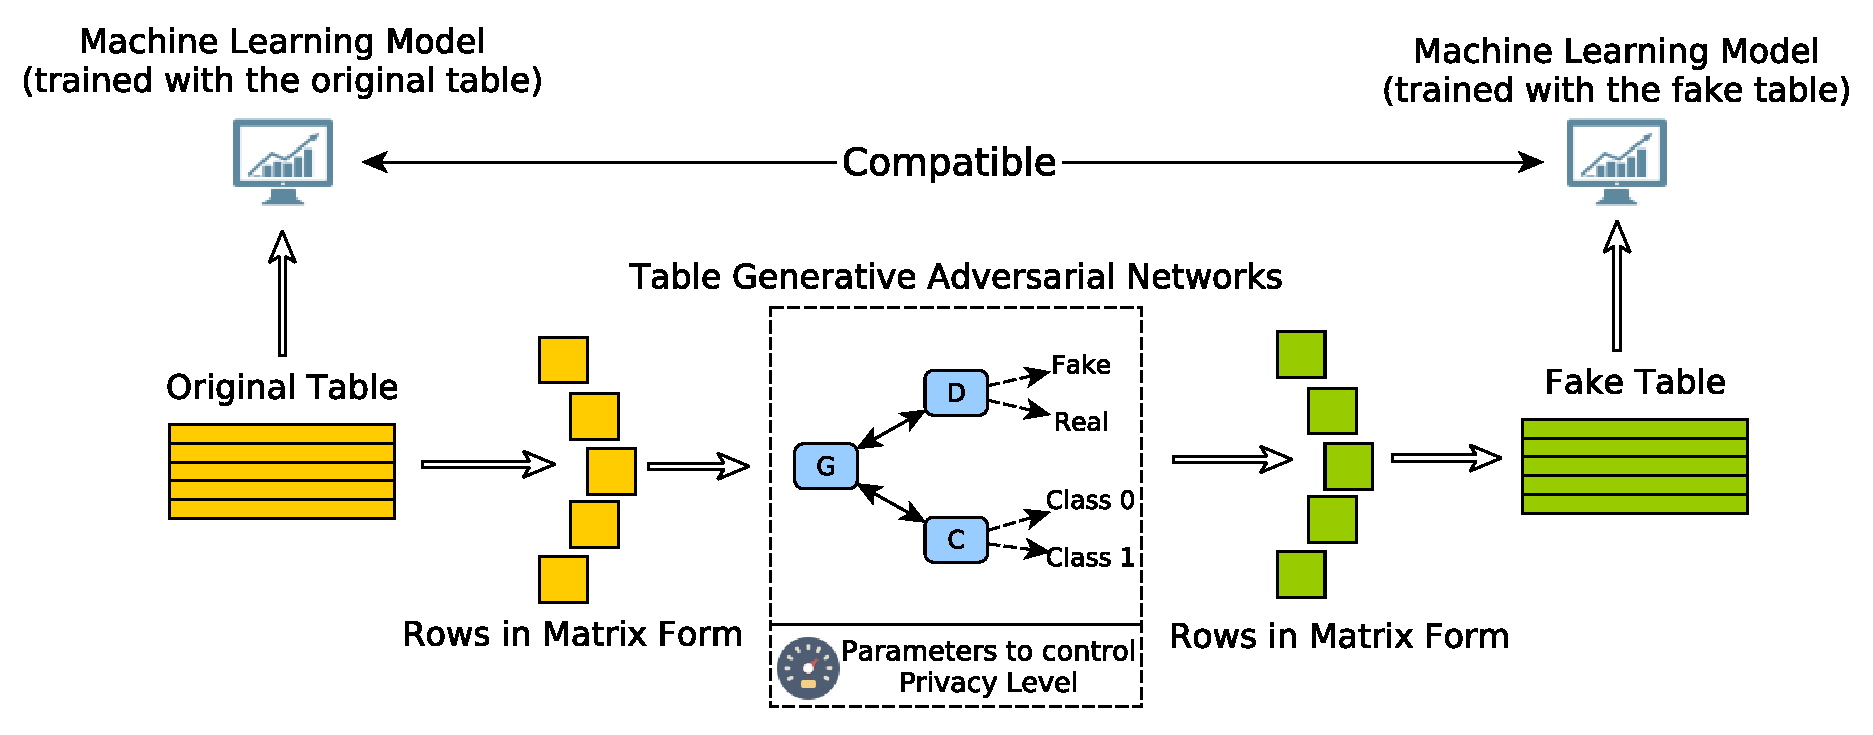
\includegraphics[width=0.8\textwidth]{tableGAN.eps}
\vspace{-1em}
\caption{The overall workflow of the proposed method. The fake table (marked in green) is generated by the proposed table-GAN trained using the original table (marked in yellow). Machine learning models trained using the fake table should show the same behaviors as models trained using the original table (i.e., model compatibility). Our goal is to achieve general model compatibility regardless of machine learning algorithms and tasks.}
\label{fig:tablegan}
\end{figure*}
% Existing data anonymization techniques remove identifying attributes of a table and transform quasi-identifiers (QIDs) using generalization \cite{samarati_2001_protecting}, micro-aggregation \cite{domingo_2005_ordinal,domingo_2002_practical}, etc.For example, Table~\ref{T:mot_origintable} shows an original table and Table~\ref{T:mot_anonymized} is its anonymized version using $k$-anonymity and $t$-closeness. In this example, ZIP code and age are QIDs, and salary and disease are sensitive attributes. As Table~\ref{T:mot_anonymized} shows, only QIDs are transformed and the sensitive attributes have their initial values.
% Existing data anonymization techniques remove identifying attributes of a table and transform quasi-identifiers (QIDs) using generalization \cite{samarati_2001_protecting}, micro-aggregation \cite{domingo_2005_ordinal,domingo_2002_practical}, etc. These techniques do not change values in sensitive attributes but only QIDs to satisfy a criteria requested by a privacy model such as $k$-anonymity or $t$-closeness. This means that the sensitive values are left intact in the anonymized table to maintain the usability in future analyses. For example, Table~\ref{T:mot_origintable} shows an original table and Table~\ref{T:mot_anonymized} is its anonymized version using $k$-anonymity and $t$-closeness. In this example, ZIP code and age are QIDs, and salary and disease are sensitive attributes. As Table~\ref{T:mot_anonymized} shows, only QIDs are transformed and the sensitive attributes have their initial values.

% Researchers in \cite{soria_2013_differential} and \cite{sun_2011_extended} have mentioned that while t-closeness can partially address the attribute disclosure problem, it can lead to noticeable utility losses in high dimensional data by breaking the link between the sensitive attributes and quasi-identifiers.
% , which is a main also applicable for $\epsilon$-differential privacy \cite{soria_2014_enhancing}.
% Other perturbation methods can change sensitive values. However, they are not proved for general model compatibility. In terms of model compatibility, anonymization is better than perturbation. See \cite{brickell_2008_cost} and \cite{domingo_2008_critique} for more detailed critiques about the shortcomings of current privacy models in the attribute disclosure problem.

% \textbf{We want to generate a synthetic table that does not contain any real information but its usability is maintained in future tasks such as classification and regression.} Recent achievements in generative models by the deep learning community enable this idea.

% \subsection{Problem Statement}
%  One more drawback of them is that a one-to-one relationship exists between the original table and the anonymized/perturbed table, and re-identification attacks are possible after discovering this relationship.
% Existing data anonymization/perturbation methods are not perfect because i) there is a chance of leaking sensitive information (i.e., attribute disclosure) and ii) a one-to-one relationship exists between the original table and the anonymized/perturbed table, and re-identification attacks are possible after discovering this relationship.

\begin{table}[t]
\small
\caption{Original Table. ZIP and Age are QIDs; Salary and Disease are sensitive attributes.}
\label{T:mot_origintable}
\vspace{-1em}
\begin{center}
\begin{tabular}{| c | c | c | c | c | }
\hline
No  & ZIP & Age & Salary & Disease \\
\hline
1 & 47677 &  29 & 3K &  AIDS  \\ 
2 & 47672 &  22 & 4K &  Ebola \\ 
3 & 47678 &  27 & 5K &  Cancer  \\ 
4 & 47905 &  53 & 6K &  AIDS  \\ 
5 & 47909 &  52 & 11K &  Ebola  \\  
6 & 47906 &  57 & 8K &  Heart Disease  \\  
% 7& 47605 &  30 & 7K &  Heart Disease  \\ 
% 8 & 47673 &  36 & 9K &  Ebola  \\  
% 9 & 47607 &  32 & 10K &  Cancer  \\ 
\hline
\end{tabular}
\end{center}
\caption{Table anonymized by 3-anonymity and 3-diversity. There are two equivalence classes and in each equivalence class, there are three records that are not distinguishable w.r.t. QIDs (i.e., 3-anonymity) and their sensitive values are all different (i.e., 3-diversity). \label{T:mot_anonymized}}
\vspace{-1em}
\begin{center}
\begin{tabular}{| c | c | c | c | c | }
\hline
No  & ZIP & Age & Salary & Disease \\
\hline
1 & 4767* &  $\leq$ 40 & 3K &  AIDS  \\ 
2 & 4767* &  $\leq$ 40 & 4K &  Ebola  \\ 
3 & 4767* &  $\leq$ 40 & 5k &  Cancer \\ \hline
4 & 4790* &  $\geq$ 50 & 6K &  AIDS  \\ 
5 & 4790* &  $\geq$ 50 & 11K &  Ebola  \\  
6 & 4790* &  $\geq$ 50 & 8K &  Heart Disease  \\ \hline
% 7& 4760* &  $\leq$ 40 & 4K &  Ebola  \\ 
% 8 & 4760* &  $\leq$ 40 & 7K &  Heart Disease   \\  
% 9 & 4760* &  $\leq$ 40 & 10K &  Cancer  \\  \hline
\end{tabular}
\end{center}
\end{table}

% \textbf{Our goal is to generate fake tables that show very good balance between them. In our fake table, there is no one-to-one correspondence. All identifiers, QIDs and sensitive attributes are fabricated by the proposed table-GAN}.

\subsection{Overall Workflow}
The overall workflow of our approach is presented in Figure~\ref{fig:tablegan}. It is processed in the following sequence:

\begin{itemize}
\item Records in the original table are converted into square matrix form; if needed, we pad with zeros. For example, a record that consists of 24 values can be converted into a $5 \times 5$ square matrix after padding a zero.
\item The proposed table-GAN is trained using the converted square matrices --- we will describe the details of the table-GAN in Section~\ref{sec:approach}.
\item The table-GAN generates many synthetic square matrices (i.e., synthetic records) that will be converted and merged into a table.
\item The generated fake table is shared with partners who will perform analyses and design machine learning models.
\item \textbf{The machine learning model trained using the synthetic table should be able to replace the model trained using the original table. In particular, we call this property \textit{model compatibility}.}
\end{itemize}

The generation process should have parameters to trade off between the level of privacy and the model compatibility. By decreasing the level of privacy, we can make records in the synthetic table similar to records in the original table and improve model compatibility.

\subsection{Data Types}
Our method is able to generate categorical, discrete and continuous values. Essentially, our model generates only continuous numerical values. For discrete values, however, we perform rounding at the final generation stage to convert continuous values into discrete values. For categorical values, the process is the same as for the discrete numerical values after label encoding (i.e., assigning an integer number to each category).%Editor: Please ensure that the intended meaning has been maintained in the above edit.

Table~\ref{T:example} presents an example that the proposed table-GAN is able to work with. SSN is a global identifier, gender and age are QIDs, cholesterol and diabetes are sensitive attributes, and in particular, diabetes contains ground-truth labels that can be used for model compatibility tests.

\begin{table}[t]
\small
\caption{An example table that can be synthesized by the proposed table-GAN\label{T:example}}
\vspace{-1em}
\begin{center}
\begin{tabular}{| c | c | c | c | c | }
\hline
SSN  & Gender & Age & Cholesterol & Diabetes \\
\hline
1 & Male &  29 & 65.5 &  0  \\ 
2 & Male &  22 & 130.9 &  1 \\ 
3 & Female &  27 & 190.1 &  1  \\ 
4 & Female &  43 & 78.4 &  0  \\
\hline
\end{tabular}
\end{center}
\end{table}

We leave other data types as future work. For instance, hierarchical recurrent neural networks are able to process a table that consists of string attributes~\cite{ElHihi:1995:HRN:2998828.2998898}. To our knowledge, there are no attempts to generate both of continuous numerical values and discrete strings within a single model.
\section{Proposed Method}\label{sec:approach}
% \begin{figure*}[t]
% \centering
%   \includegraphics[width=0.5\textwidth]{gcdArch.jpg}
%   \caption{GAN Architecture}
%   \label{fig:gcdarch}
%   \vspace{20pt}%
% \end{figure*}

\begin{figure*}[t]
\centering
\includegraphics[width=0.7\textwidth]{GAN-Dicriminator.png}
\vspace{-1em}
\caption{Our table-GAN architecture. The classifier is omitted because of space limitations, and it has the same neural network architecture as the discriminator. The generator (resp. discriminator) performs a series of deconvolution (resp. convolution) operations to generate (resp. classify) a record. The final loss after the sigmoid activation can be back-propagated to the generator. The dimensions of the latent vector input $z$ and intermediate tensors should be configured considering the number of attributes (e.g., $16 \times 16=196$ attributes in this figure).}
  \label{fig:gdlayers}
\end{figure*}

We introduce the proposed table-GAN that, given a table to synthesize and several parameters to control the privacy level, generates a synthetic table that is statistically similar to the original table.


\subsection{Neural Network Architecture}
The deep convolutional GAN (DCGAN) is one of the most influential works for GANs. Many meaningful ideas have been proposed to design the neural network architecture of the generator ($G$) and the discriminator ($D$), as follows: (1) replacing spatial pooling functions with strided convolutions, (2) eliminating fully connected hidden layers, and (3) using batch normalization~\cite{conf/icml/IoffeS15}, ReLU for the generator~\cite{icml2010_NairH10}, and LeakyReLU~\cite{maas2013rectifier} for the discriminator.

Our model also adopts the DCGAN architecture but has an additional neural network called \textit{classifier} ($C$), as follows:
\begin{itemize}
\item A generator neural network $G$ to produce synthetic records that have the same distribution as that of real records;
\item A discriminator neural network $D$ to distinguish between real and synthetic records;
\item A classifier neural network $C$ to predict synthetic records' labels. We found that adding $C$ helps maintain the consistency of values in the generated records. For instance, a record with gender = ``Male'' and disease = ``Uterine Cancer''  can be prevented; the classifier learns about the consistency from the original table.
\end{itemize}

We describe neural network architectures in more detail in the following.
% GANs basically contain two competing neural networks. One of these networks generates samples and the other one discriminates the real samples from the generated ones. These two networks are trained simultaneously until they converge to a point that the generated samples can not be distinguished from real ones with high confidence.  
% functions....

\subsubsection{Discriminator}
The discriminator network $D$ is a neural network trained to classify the generated records as \textit{synthetic} and the records in the original table as \textit{real}. 
% The inputs to this network are training data form the original dataset and the generated samples from the generator component. 
Precisely, $D$ is a convolutional neural network (CNN) that contains multiple layers. In each layer, a list of learnable filters (e.g., 3$\times$3 matrices) are applied to the entire input matrix (i.e., convolution operations). Recall that records are converted into square matrices in our method. Thus, the layer output size is proportional to the number of filters in each layer.

The output of a layer is the input to the next layer, as shown in Figure~\ref{fig:gdlayers}. The dimension of intermediate tensors keeps decreasing and the depth continues increasing until the last sigmoid activation layer that generates the probability of being real or synthetic. There are other intermediate layers (omitted in Figure~\ref{fig:gdlayers}) that affect the functionality of the network, such as batch normalization or LeakyReLU~\cite{radford_dcgan_2015}.

% Each filter has different parameters (weights and biases) to be learned and these learnable parameters are tuned during the back-propagation mechanism\cite{}. Back-propagation is an iterative learning mechanism which starts from the last layer and backwards the initial layers to tune the parameters of the each layer in order to reach the best prediction results out of the neural network. The learning process needs a metric to measure the efficiency of the learning steps. Loss or cost functions are used to measure the differences between the current outcome of the neural network and the desired results. The goal of the training mechanisms is to find the best values for parameters of the neurons by minimizing the loss functions. The learning algorithms achieve these goal by using the descending gradients(vector of partial derivatives) of the loss functions to calculate the new values for the parameters in each learning iteration. We utilizes the standard learning technique used in the neural networks called Stochastic Gradient Descent(SGD) which uses a small randomly selected portion of the training data to calculate the gradients. We also use the Adam algorithm \cite{} as the optimizer algorithm for the SGD technique.\\

The input to the first layer is a $d \times d$ matrix that represents one real or synthetic record. The discriminator is trained to predict 1 for real records and 0 for synthetic records after the last sigmoid layer.

If the number of attributes in the original table is less than the input size, then each record is padded with zeros and reshaped into a square matrix. Our model is configurable and able to learn from a table with many attributes (e.g., $16 \times 16 = 256$ attributes in a single table and some GANs supports images that are as large as $1024 \times 2014$~\cite{2017arXiv171010196K}).
% To minimize the side-effects of the zero-padding, we duplicate records multiple times and minimize the number of padded zeros.   
% The feature of the input samples ( form both training data and generated samples) will be extracted through the convolutional layers and the final layer uses the activation functions to generate the probability of being fake or real. 

% D Shape image : (64, 8, 8, 1)
% D Shape h0: (64, 4, 4, 3)
% D Shape h1: (64, 2, 2, 66)
% D Shape h3: (64, 1)

% G shape z : (64, 100)
% G Shape h0: (64, 1, 1, 256)
% G Shape h2: (64, 2, 2, 128)
% G Shape h3: (64, 4, 4, 64)
% G: Shape h4: (64, 8, 8, 1)

\subsubsection{Generator}
The generator $G$ is also a neural network that consists of multiple de-convolutional layers. As shown in Figure~\ref{fig:gdlayers}, $G$ performs a process that is opposite to that of the discriminator. Its input is a latent vector $z$ that is uniformly sampled from the unit hypercube space\footnote{A high-dimensional space where each dimension is confined to the range of [-1,1]}. Multiple de-convolutional layers convert the input $z$ to a 2-dimensional matrix corresponding to a record in the synthetic table.

The generator can be trained by the discriminator's prediction result (in fact, this is one of the multiple ways we propose to train the generator in our table-GAN). Its goal is to deceive the discriminator. This training process can be very efficiently implemented by back-propagation.
% In fact, the generator learns the features of the training dataset in respect to its attributes(columns) in a MinMax game mechanism.  In this mechanism the generator network's parameters are repeatedly (learning process contains many iterations) tunned in such way that the generated samples can fool the discriminator to classify them as real ones with the lowest possible error rate in each iteration. The parameter tuning mechanism is based on the traditional back-propagation techniques used in neural networks. We use the Stochastic Gradient Descent(SGD) as the learning optimization technique. More  here ... //

% The training algorithms aims to train G to be a good estimator of training data(x).
% The convolutional layers in the generator component

% by propagating the errors to  rate to the  learning mechanism is is done using the back propagation mechanism and the learning optimization techniques such as SGD.
% At the end of training the generator is in a state that can generate desired samples similar to the original dataset.
% Is it correct this way? More details about the convolutional layers, and their dimensions?

\subsubsection{Classifier}\label{sec:class}
The classifier network $C$ has the same neural network architecture as the discriminator. However, it is trained by ground-truth labels in the original table. In Table~\ref{T:example}, for instance, the diabetes attribute contains ground-truth labels. Therefore, the classifier is trained to learn about the correlation between the cholesterol and diabetes attributes from the table. Given a synthetic record, it can teach the generator whether the record is semantically correct. For example, (cholesterol=50, diabetes=1) is not a correct record because cholesterol=50 is too low to be diagnosed as diabetes. If such records are synthesized by the generator, the classifier can effectively correct the generator.

In fact, the discriminator itself can learn about the semantic integrity to some degree. Semantically incorrect generations are likely not to be classified as real by the discriminator. However, it does not mainly consider about the semantic integrity and we found some incorrect generation examples without the classifier.


\subsection{Loss Functions}
The loss function contains the philosophy for training neural networks. In general, neural networks are trained by minimizing a loss function, and ill-designed loss functions deteriorate the training process and lead to malfunctioning neural networks. Therefore, the design of loss functions to train the three proposed neural networks is key for successful table syntheses. We adopt one loss function from DCGAN and design two more loss functions, as follows:

\begin{enumerate}
\item The \textit{original loss} is adopted from DCGAN and was already shown in Equation~\ref{eq:gan}.
\item The \textit{information loss} is defined as the discrepancy between two statistics of synthetic and real records.
\item The \textit{classification loss} is defined as the discrepancy between the predicted label by the classifier and the synthesized label.
\end{enumerate}

% Loss functions determines 

% In the remaining of the paper we use the following notation
% and terminology:
% X - the clean training data from the dataset.
% y : the label for training data
% J(X, y): the cost function to be minimized for training.

\textbf{The discriminator is trained with the original DCGAN loss, and the classifier is trained with the classification loss. The generator is trained with all three loss functions because it is the most important neural network in our method.} In this subsection, we introduce the individual loss functions.

\subsubsection{Original Loss}
The original DCGAN loss function is shown in Equation~\ref{eq:gan}. The discriminator is trained to maximize it, and the generator is trained to minimize it. It represents the training philosophy of GANs (i.e., while the generator attempts to deceive the discriminator, it can significantly improve its synthesis capability). See~\cite{goodfellow2014generative,radford_dcgan_2015} for more detailed descriptions of the original loss. There are also some variations of the original loss~\cite{2017arXiv170104862A}, but the most widely used one is still the one we already introduced.

The exact loss function to train the discriminator can be written as follows:
\begin{equation}\label{eq:origD}\begin{aligned}
\Loss_{orig}^{D} = & -\mathbb{E}[\log D(x)]_{x \sim p_{data}(x)} \\
  & - \mathbb{E}[\log (1-D(G(z)))]_{z \sim p(z)},
\end{aligned}\end{equation}
and the generator can be written as follows:
\begin{equation}\label{eq:origG}\begin{aligned}
\Loss_{orig}^{G} = \mathbb{E}[\log (1-D(G(z)))]_{z \sim p(z)}.
\end{aligned}\end{equation}

Note that we added negative signs in $\Loss_{orig}^{D}$ to convert the maximization of Equation~\ref{eq:gan} to the minimization. Deep learning algorithms typically prefer to minimize losses. There are multiple different ways to implement the loss in program codes but it is usually calculated using cross entropy\footnote{One example is the DCGAN implementation in \url{https://github.com/carpedm20/DCGAN-tensorflow/blob/251aa440013afb86ddfefef8ddce3629be7972ac/model.py#L124}.}.

\subsubsection{Information Loss}
To define the information loss, we extract features immediately before the sigmoid activation of the discriminator network (i.e., the flattened tensor marked in yellow in Figure~\ref{fig:gdlayers}). From these features, the discriminator decides whether the inputs are real or synthetic. Thus, \textbf{it is reasonable to say that the extracted features contain key characteristics of the input samples}. In general, extracted features become very high-dimensional vectors after flattening. We use bold font $\f$ to denote these vectors.

The simplest form of information loss is as follows:
\begin{equation}\label{eq:mean}\begin{aligned}
\Loss_{mean} =  & \| \mathbb{E}[\f_x]_{x \sim p_{data}(x)} - \mathbb{E}[\f_{G(z)}]_{z \sim p(z)}\|_2,
\end{aligned}\end{equation}
where $\f$ stands for features (i.e., high-dimensional vectors) extracted from the last layer of the discriminator and $\mathbb{E}[\f]$ means the average feature (i.e., the centroid of the vectors) of all records in the dataset. Note that we use the L-2 norm (Euclidean norm) to measure the discrepancy between two mean features (vectors).

Thus, $\Loss_{mean}$ is to compare the first-order statistics (i.e., mean) of the features of real and synthetic records. We also use the second-order statistics (i.e., standard deviation) as follows:
\begin{equation}\label{eq:std}\begin{aligned}
\Loss_{sd} =  & \| \mathbb{SD}[\f_x]_{x \sim p_{data}(x)} - \mathbb{SD}[\f_{G(z)}]_{z \sim p(z)}\|_2,
\end{aligned}\end{equation}
where $\mathbb{SD}[\cdot]$ represents the standard deviation of features.

$\Loss_{mean}=0$ and $\Loss_{sd}=0$ mean that real and synthetic records  have the statistically same features from the perspective of the discriminator (recall that the extracted features are from the last layer of the discriminator). This further implies that the discriminator may not be able to distinguish them.

\textbf{The quality of the synthesis process should be controllable}. With unreliable partners, you may not want to share a synthetic table that is very similar to the original table. You may want to intentionally generate a low-quality table in that case. For this purpose, we design the following loss to train the generator based on the hinge-loss that does not incur any loss until a predetermined quality degradation threshold:
\begin{equation}\begin{aligned}
\Loss_{info}^{G} =  & \max(0, \Loss_{mean}-\delta_{mean}) + \max(0, \Loss_{sd}-\delta_{sd}).
\end{aligned}\end{equation}

The information loss $\Loss_{info}^G$ provides zero loss as long as $\Loss_{mean}$ (resp. $\Loss_{sd}$) is smaller than a threshold $\delta_{mean}$ (resp. $\delta_{sd}$). Thus, $\delta_{mean}$ and $\delta_{sd}$ are two parameters for controlling the level of privacy. If these parameters are small, then the privacy level will be lower, and the synthetic table will be similar to the original table.

\subsubsection{Classification Loss}
We found that  values occasionally do not match with labels in synthetic records, as stated in Section~\ref{sec:class}. To avoid this situation, we design an additional loss function called \textit{classification loss}, as follows:
\begin{equation}\label{eq:class}\begin{aligned}
\Loss_{class}^{C} =  & \mathbb{E}[|\ell(x)-C(remove(x))|]_{x \sim p_{data}(x)},
\end{aligned}\end{equation}
\begin{equation}\begin{aligned}
\Loss_{class}^{G} = &\mathbb{E}[|\ell(G(z))-C(remove(G(z)))
|]_{z \sim p(z)},
\end{aligned}\end{equation}
where $\ell(\cdot)$ is a function that returns the label attribute value of an input record, $remove(\cdot)$ is to remove the label attribute of an input record, and $C(\cdot)$ is a label predicted by the classifier neural network. Thus, this loss is to measure the discrepancy between the label of a generated record and the label predicted by the classifier for that record.

We also found that synthetic records occasionally do not recall all values in the original table. For instance, a certain small range of age in Table~\ref{T:example} is never generated even after setting $\delta_{mean}=0$ and $\delta_{sd}=0$ (i.e., the lowest privacy level and the highest quality in synthetic records). Surprisingly, we discovered in our experiments that the proposed classification loss is able to somehow address this problem in many cases. This is one additional advantage of using the classification loss.

\subsection{Training Algorithm}
In this subsection, we will describe the training algorithm of the proposed table-GAN. In practice, we cannot train neural networks after loading all records simultaneously due to GPU memory limitations. Thus, deep learning algorithms that work with large datasets use the stochastic gradient descent (SGD) update based on mini-batches. We also adopt this approach for better scalability.

However, one problem in the mini-batch training is that we cannot directly calculate the global mean and standard deviation of real and synthetic samples' features (recall that $\Loss_{mean}$ and $\Loss_{sd}$ require them). Thus, we use the exponentially weighted moving average to approximate them (lines~\ref{alg:mva1}$\sim$\ref{alg:mva2} of Algorithm~\ref{alg:tgan}). For instance, $\mathbb{E}[\f_x]_{x \in X_{mini}}$ (resp. $\mathbb{E}[\f_{G(z)}]_{z \in Z_{mini}}$) means the mean feature of real (resp. synthetic) mini-batch records. Using them, it calculates the global mean features $\f_{mean}^X$ and $\f_{mean}^Z$. In general, the weight $w$ should be close to 1 in the moving average calculation to have the stable global mean and standard deviation of features (we used $w=0.99$).

All loss functions should be rewritten considering the mini-batch training as follows:
\begin{equation}\begin{aligned}
\Loss_{orig}^{D} = & -\mathbb{E}[\log D(x)]_{x \in X_{mini}} \\
  & - \mathbb{E}[\log (1-D(G(z)))]_{z \in Z_{mini}},
\end{aligned}\end{equation}
\begin{equation}\begin{aligned}
\Loss_{orig}^{G} = \mathbb{E}[\log (1-D(G(z)))]_{z \in Z_{mini}},
\end{aligned}\end{equation}
\begin{equation}\begin{aligned}
\Loss_{mean} =  & \| \f_{mean}^X - \f_{mean}^Z\|_2,
\end{aligned}\end{equation}
\begin{equation}\begin{aligned}
\Loss_{sd} =  & \| \f_{sd}^X - \f_{sd}^Z\|_2,
\end{aligned}\end{equation}
\begin{equation}\begin{aligned}
\Loss_{class}^{C} =  & \mathbb{E}[|\ell(x)-C(remove(x))|]_{x \in X_{mini}},
\end{aligned}\end{equation}
\begin{equation}\begin{aligned}
\Loss_{class}^{G} = &\mathbb{E}[|\ell(G(z))-C(remove(G(z)))
|]_{z \in Z_{mini}}.
\end{aligned}\end{equation}

The training sequence in an epoch is i) training the discriminator with $\Loss_{orig}^{D}$ (line~\ref{alg:d2}), ii) training the classifier with $\Loss_{class}^{C}$ (line~\ref{alg:c2}), and iii) training the generator with $\Loss_{orig}^{G} + \Loss_{info}^{G} + \Loss_{class}^{G}$ (line~\ref{alg:g2}).

\begin{algorithm2e}[!t]
% \footnotesize
\DontPrintSemicolon
\hrule
\KwIn{real records: $\{x_1, x_2, \cdots\} \sim p(x)$}
\KwOut{a generative model $G$}
\hrule
$G \gets$ a generative neural network\;
$D \gets$ a discriminator neural network\;
$C \gets$ a classifier neural network\;
\tcc{Initializing to zero vectors}
$\f_{mean}^X \gets \mathbf{0}$;
$\f_{sd}^X \gets \mathbf{0}$;
$\f_{mean}^Z \gets \mathbf{0}$;
$\f_{sd}^Z \gets \mathbf{0}$\;
\While{until convergence of loss values} {
Create a mini-batch of real records $X_{mini}= \{x_1,\cdots,x_n\}$\;
Create a mini-batch of latent vector inputs for $G$ $Z_{mini} = \{z_1,\cdots,z_n\}$\;

Perform the SGD update of the discriminator $D$ with $\Loss_{orig}^{D}$\;\label{alg:d2}

Perform the SGD update of the classifier $C$ with $\Loss_{class}^{C}$\;\label{alg:c2}
\tcc{Moving average update of the mean and standard deviation of features}

$\f_{mean}^X = w \times \f_{mean}^X + (1-w) \times \mathbb{E}[\f_x]_{x \in X_{mini}}$\;\label{alg:mva1}
$\f_{sd}^X = w \times \f_{sd}^X + (1-w) \times \mathbb{SD}[\f_x]_{x \in X_{mini}}$\;

$\f_{mean}^Z = w \times \f_{mean}^Z + (1-w) \times \mathbb{E}[\f_{G(z)}]_{z \in Z_{mini}}$\;
$\f_{sd}^Z = w \times \f_{sd}^Z + (1-w) \times \mathbb{SD}[\f_{G(z)}]_{z \in Z_{mini}}$\;\label{alg:mva2}

Perform the SGD update of the generator $G$ with $\Loss_{orig}^{G} + \Loss_{info}^{G} + \Loss_{class}^{G}$\;\label{alg:g2}

}
\Return $G$\;
\hrule
\caption{\strut Training algorithm of table-GAN.\label{alg:tgan}}
\end{algorithm2e}

Calculating the theoretical complexity for deep learning algorithms is rather cumbersome and meaningless because its training involves many neural networks and gradients of loss functions (that can be accelerated by GPUs). However, our algorithm requires at most 20 minutes of training time in our experiments.

\subsection{How to generate synthetic records}
We described how to train the proposed table-GAN. In this subsection, we explain how to generate synthetic records from the trained model.

As shown in Figure~\ref{fig:gdlayers}, the input to the generator is a latent vector $z$. We first randomly sample $z$ in the unit hypercube space and input it to the generator. Its output is one synthetic record. Thus, the generation process is very simple and lightweight compared to the training process.

\subsection{Scalability Issue}\label{scal}
There are several standard methods to increase the scalability of deep learning algorithms. Tensorflow supports distributed learning by default and without large efforts, and we can extend to a distributed synthesis method. DownpourSGD, ADMM, EASGD, and GoSGD (all of which are well summarized in~\cite{DBLP:journals/corr/Zhang16b}) are other famous general distributed learning algorithms. Extensions based on these approaches are also straightforward. An additional advantage of using these approaches is that they perform \textit{ranged-based} search rather than \textit{point-based} search during SGD updates. For the difference between range-based and point-based search, refer to~\cite{Boyd:2011:DOS:2185815.2185816}.

Another approach to increase the scalability is to i) split a table into several smaller chunks, ii) train a table-GAN with each chunk independently, and iii) generate records with each trained table-GAN and merge them into a synthetic table. \textbf{Its runtime linearly decreases w.r.t. the number of chunks in this approach.} We used this method to synthesize large tables in our experiments.
\section{Experimental Analysis}
We describe the experimental environments and results. We have chosen four tables from four domains: payroll, health, personal records, and airline market. The baseline methods are anonymization\slash perturbation techniques implemented in ARX\footnote{One of the most popular tools accessible in \url{http://arx.deidentifier.org}} and sdcMicro\footnote{An open-source tool comparable to $\mu$-ARGUS. Accessible in \url{https://cran.r-project.org/web/packages/sdcMicro/index.html}}, and other generative models. Throughout the experiments, our table-GAN shows the best balance between privacy level and model compatibility.

\subsection{Experimental Environments}
\subsubsection{Dataset} We use four tables, as summarized in Table~\ref{T:data}. The LACity dataset\footnote{\url{https://controllerdata.lacity.org/Payroll/City-Employee-Payroll/pazn-qyym}} contains records of Los Angeles city government employees (such as salary, department and so on). The Adult dataset\footnote{\url{https://archive.ics.uci.edu/ml/machine-learning-databases/adult}} has many personal records (such as nationality, education level, occupation, work hours per week, and so forth). The Health dataset\footnote{\url{https://wwwn.cdc.gov/Nchs/Nhanes/Default.aspx}} consists of various information (such as blood test results, questionnaire survey, diabetes, and so on). The Airline dataset is created by the Bureau of Transportation Statistics (BTS). BTS randomly selects 10\% of all tickets sold in the USA and releases these data to the public every quarter\footnote{\url{https://www.transtats.bts.gov/DataIndex.asp}}. Each dataset has one ground-truth label that can be used for model compatibility tests, as follows:
\begin{enumerate}
\item In the LACity dataset, we know the salary information of employees. Thus, regression analysis tests are available. For classification tests, we use the median salary and create the high-salary attribute.  If an employee is paid more than the median salary, then its label is 1.
\item In the Adult dataset, the work-hour attribute has the information of work hours per week for each individual. We create additional binary labels after checking whether people work longer than the median case. Thus, we perform both classification and regression tests with this dataset.
\item In the Health dataset, we have the diabetes attribute, which indicates whether a person has been diagnosed as having diabetes by doctors. Only classification tests are available in this dataset.
\item In the Airline dataset, there is an attribute that contains ticket price information. We can perform regression tests with this attribute. We also create binary labels of whether prices are greater than the median price for classification tests.
\end{enumerate}

We generate synthetic tables that have the same number of records as the original table. For each dataset, we also prepared for testing records that are not part of the original table to check the model compatibility. The number of testing records is approximately 20\% of the number of records in the original table.

\begin{table}[t]
\centering
\small
\caption{Statistics of datasets\label{T:data}}
\begin{tabular}{|c|c|c|c|c|}
\hline
        & \# of Records & \# of QIDs & \begin{tabular}[c]{@{}c@{}}\# of Sensitive\\ Attributes\end{tabular} & \begin{tabular}[c]{@{}c@{}}\# of Testing\\ Records\end{tabular} \\ \hline
LACity &    15000  &    2  &     21   &   3000      \\ \hline
Adult   &    32561 &     5       &      9    &   16281   \\ \hline
Health  &    9813 &      4      &       28 &     1963  \\ \hline
Airline  &    1000000   &   2    &    30  &     200000  \\ \hline
\end{tabular}

\centering
\caption{Training time of table-GAN in each dataset. We used the multi-chunk parallel approach for Airline to save its training and generating time (see Section~\ref{scal}).\label{T:time}}
\begin{tabular}{|c|c|c|c|c|}
\hline
   & LACity & Adult  & Health & Airline \\ \hline
\begin{tabular}[c]{@{}c@{}}Training Time of\\ table-GAN\end{tabular} & 3.9 mins  & 8.16 mins & 1.9 mins & 20.2 mins \\ \hline
\end{tabular}

\scriptsize
\centering
\caption{Euclidean distance between a real record to its closest synthetic/anonymized/perturbed record after attribute-wise normalization. Its format is $\textrm{average} \pm \textrm{std dev}$ in each cell. Risky cases, where the average distance is too small or the standard deviation is too large, are indicated in red.\label{T:dist}}
\begin{tabular}{|c|c|c|c|c|c|}
\hline
       & \begin{tabular}[c]{@{}c@{}}table-GAN\\ (low-privacy)\end{tabular} & \begin{tabular}[c]{@{}c@{}}table-GAN\\ (high-privacy)\end{tabular} & \begin{tabular}[c]{@{}c@{}}The best of\\ARX\end{tabular} & \begin{tabular}[c]{@{}c@{}}The best of\\sdcMicro\end{tabular} & DCGAN \\ \hline
\multicolumn{6}{|c|}{QIDs + Sensitive attributes} \\ \hline
LACity & $0.96 \pm 0.22$ & $1.48 \pm 0.3$ & {\color{red}$0.68 \pm 0.52$} & {\color{red}$0.07 \pm 0.17$} & $0.83 \pm 0.31$   \\ \hline

Adult  & $0.75 \pm 0.19$ & $1.84 \pm 0.23$ & $0.59\pm0.17$ & $0.54 \pm 0.12$ & $0.88 \pm 0.24$     \\ \hline

Health & $2.53 \pm 0.43$ & $2.75 \pm 0.41$ & $0.61 \pm 0.25$ & $1.23 \pm 0.34$ & $2.85 \pm 0.42$ \\ \hline

Airline & $1.21 \pm 0.21$ & $1.23 \pm 0.27$ & $1.46 \pm 0.32$ & {\color{red}$0.98 \pm 0.41$} & $0.86 \pm 0.15$ \\ \hline

\multicolumn{6}{|c|}{Only Sensitive attributes} \\ \hline

LACity & $0.68 \pm 0.18$ & $1.24 \pm 0.17$ & {\color{red}$0 \pm 0$} & {\color{red}$0.05 \pm 0.13$} & $0.54 \pm 0.18$ \\ \hline

Adult  & $0.45 \pm 0.14$ & $1.25 \pm 0.17$ & {\color{red}$0 \pm 0$} & {\color{red}$0.2 \pm 0.1$} & $0.82 \pm 0.24$  \\ \hline
 
Health & $2.4 \pm 0.38$ & $2.56 \pm 0.39$ & {\color{red}$0 \pm 0$} & {\color{red}$0.22 \pm 0.2$ } & $2.68 \pm 0.41$  \\ \hline

Airline & $0.96 \pm 0.19$ & $1.08 \pm 0.26$ & {\color{red}$0 \pm 0$} & {\color{red}$0.69 \pm 0.36$} & $0.76 \pm 0.16$ \\ \hline
\end{tabular}
\end{table}

\subsubsection{Evaluation Method} The evaluation of data anonymization, perturbation and synthesis methods cannot be performed in a simple manner. This evaluation involves several different methods because they should be evaluated in various aspects. We use the following three evaluation methods:

\begin{enumerate}
\item \textit{Statistical comparison} is to compare statistical similarity between an attribute in the original table and a corresponding attribute in anonymized\slash perturbed\slash synthesized tables. We will compare cumulative distributions and histograms for each attribute.
\item \textit{Distance to the closest record (DCR)} means Euclidean distance between a record $r$ of an anonymized\slash perturbed\slash synthesized table and the closest record to $r$ in the original table. Note that an anonymized\slash perturbed\slash synthesized record with DCR = 0 leaks real information. We calculate the distance after attribute-wise normalization because each attribute contributes to the distance equally after the normalization. Distance-based metrics are widely used in many works~\cite{Mateo-Sanz2004}. There also exist several risk evaluation metrics~\cite{Domingo-ferrer01comparingsdc,Mateo-Sanz04outlierprotection}. However, they require equivalence classes and one-to-one correspondence between real records and anonymized\slash perturbed\slash synthesized records. Our method does not provide them.
\item \textit{Machine learning score similarity} is to evaluate the model compatibility. After fixing a classification or regression algorithm and its parameter, we train with the original table or the anonymized\slash perturbed\slash synthesized table. If the accuracy values of the two cases for unknown testing cases are the same, then we can say that they are compatible. We use F-1\footnote{F-1 is the harmonic mean of precision and recall, and it is one of the most widely used metrics to evaluate classification models.} for classification tests and mean relative error (MRE) for regression tests.
\end{enumerate}

Note that in the model compatibility test, we exclude the grid search\footnote{It is a method to find the best parameter setup for machine learning algorithms; it evaluates the prediction accuracy of various parameter setups through cross-validation and returns only the best model}. Enabling the grid search during the test means that we compare only the best performing parameter setup for an algorithm. Because two models can show similar accuracy by accident after the grid search, we exclude it.

In general, classical anonymization techniques show good performance for the statistical comparison and machine learning score similarity tests because they do not actively change sensitive attributes. We demonstrate that our method significantly outperforms anonymization techniques with respect to DCR by slightly sacrificing the performance in the statistical comparison and machine learning score similarity tests. Surprisingly, our method shows better model compatibility  than anonymization techniques in some tests.

\subsubsection{Baseline Methods}
Among existing anonymization techniques, the combination of $k$-anonymity and $t$-closeness is considered to be the most basic method and is already implemented in ARX, a powerful anonymization tool that is widely used in real applications and research. ARX also has $(\epsilon,d)$-differential privacy and $\delta$-disclosure. Thus, we create two baseline methods with ARX: one is the combination of $k$-anonymity and $t$-closeness and the other is the combination of $(\epsilon,d)$-differential privacy and $\delta$-disclosure.  Recall that all these methods in ARX do not change sensitive attributes but construct equivalence classes (by altering QIDs) in a way that can meet the requirements of each privacy protection concept.

For perturbation, we will use the micro-aggregation (for QIDs) and the post-randomization method (for sensitive attributes) implemented in sdcMicro. Note that sdcMicro perturbs sensitive attributes as well.

Another baseline method is DCGAN, which is the state-of-the-art GAN model for generating images. Because we convert a record into a matrix, DCGAN is also able to synthesize records. However, their loss functions and training procedures are optimized only for images.

% Therefore, \textbf{we have four baseline methods: ARX1, ARX2, sdcMicro, and DCGAN}.

\begin{figure*}[!ht]
\centering
\subfigure[Ours,low-privacy,LACity]{\includegraphics[trim={0 0.65cm 0 0},clip,width=0.26\textwidth]{images/CO_11_00___Columns_10.png}}
\subfigure[Ours,high-privacy,LACity]{\includegraphics[trim={0 0.65cm 0 0},clip,width=0.26\textwidth]
{images/CO_11_22___Columns_10.png}}
\subfigure[DCGAN,LACity]{\includegraphics[trim={0 0.65cm 0 0},clip,width=0.26\textwidth]{images/Origin___Columns_10.png}} \\
% \subfigure[ARX1 (zero-privacy), LACity]{\includegraphics[trim={0 0.65cm 0 0},clip,width=0.24\textwidth]{LACity_ARX_10_N_01___Columns_10.png}}\\
\vspace{-1em}
\subfigure[Ours,low-privacy,Adult]{\includegraphics[trim={0 0.65cm 0 0},clip,width=0.26\textwidth]
{images/COI_11_00___Columns_2.png}}
\subfigure[Ours,high-privacy,Adult]{\includegraphics[trim={0 0.65cm 0 0},clip,width=0.26\textwidth]
{images/COI_11_22___Columns_2.png}}
\subfigure[DCGAN,Adult]{\includegraphics[trim={0 0.65cm 0 0},clip,width=0.26\textwidth]
{images/Origin___Columns_2.png}} \\
% \subfigure[sdcMicro, Adult]{\includegraphics[trim={0 0.65cm 0 0},clip,width=0.24\textwidth]
% {images/sdc_Adult___Columns_4.png}}\\
\vspace{-1em}
\subfigure[Ours,low-privacy,Health]{\includegraphics[trim={0 0.65cm 0 0},clip,width=0.26\textwidth]
{images/COI_11_00___Columns_51.png}}
\subfigure[Ours,high-privacy,Health]{\includegraphics[trim={0 0.65cm 0 0},clip,width=0.26\textwidth]
{images/COI_11_22___Columns_51.png}}
\subfigure[DCGAN,Health]{\includegraphics[trim={0 0.65cm 0 0},clip,width=0.26\textwidth]
{images/Origin___Columns_51.png}}\\
\vspace{-1em}
\subfigure[Ours,low-privacy,LACity]{\includegraphics[trim={0 0.65cm 0 0},clip,width=0.26\textwidth]
{images/CO_11_00___Column_7.png}}
\subfigure[Ours,high-privacy,LACity]{\includegraphics[trim={0 0.65cm 0 0},clip,width=0.26\textwidth]
{images/CO_11_22___Column_7.png}}
\subfigure[DCGAN,LACity]{\includegraphics[trim={0 0.65cm 0 0},clip,width=0.26\textwidth]
{images/Origin___Column_7.png}}\\
\vspace{-1em}
\subfigure[Ours,low-privacy,Airline]{\includegraphics[trim={0 0.65cm 0 0},clip,width=0.26\textwidth]
{images/tgan_low_OI_11_00___Columns_11.png}}
\subfigure[Ours,high-privacy,Airline]{\includegraphics[trim={0 0.65cm 0 0},clip,width=0.26\textwidth]
{images/tgan_high_OI_11_22___Columns_11.png}}
\subfigure[DCGAN,Airline]{\includegraphics[trim={0 0.65cm 0 0},clip,width=0.26\textwidth]
{images/dcgan_Origin___Columns_11.png}}\\
\vspace{-1em}
\caption{Cumulative distributions and histograms of sensitive attributes by DCGAN and table-GAN. X-axes are normalized. Statistics of the original attributes are marked in blue, and synthetic ones are marked in orange.}\label{fig:cd}
\end{figure*}

\subsubsection{Computing Environments}
We implemented the proposed table-GAN based on Tensorflow and trained in a server with an i7 3.4 Ghz CPU and GTX970 GPU. We did not use any expensive components for the experiments. Even in the entry-level server, it took at most 20 minutes to generate synthetic tables, as shown in Table~\ref{T:time}.

\begin{figure*}[t]
\centering
\subfigure[Ours,low-privacy,LACity]{\includegraphics[trim={1cm 0.8cm 1cm 1.37cm},clip,width=0.24\textwidth]{images/12.png}}
\subfigure[Ours,high-privacy,LACity]{\includegraphics[trim={1cm 0.8cm 1cm 1.37cm},clip,width=0.24\textwidth]
{images/10.png}}
\subfigure[The best of ARX,LACity]{\includegraphics[trim={1cm 0.8cm 1cm 1.37cm},clip,width=0.24\textwidth]{images/23.png}}
\subfigure[The best of sdcMicro,LACity]{\includegraphics[trim={1cm 0.8cm 1cm 1.37cm},clip,width=0.24\textwidth]{images/25.png}}\\
\vspace{-1em}
\subfigure[Ours,low-privacy,Adult]{\includegraphics[trim={1cm 0.8cm 1cm 1.37cm},clip,width=0.24\textwidth]{images/Adult_16.png}}
\subfigure[Ours,high-privacy,Adult]{\includegraphics[trim={1cm 0.8cm 1cm 1.37cm},clip,width=0.24\textwidth]
{images/Adult_4.png}}
\subfigure[The best of ARX,Adult]{\includegraphics[trim={1cm 0.8cm 1cm 1.37cm},clip,width=0.24\textwidth]{images/ARX_Adult_6.png}}
\subfigure[The best of sdcMicro,Adult]{\includegraphics[trim={1cm 0.8cm 1cm 1.37cm},clip,width=0.24\textwidth]{images/SDC_Adult_1.png}}\\
\vspace{-1em}
\subfigure[Ours,low-privacy,Health]{\includegraphics[trim={1cm 0.8cm 1cm 1.37cm},clip,width=0.24\textwidth]
{images/Health_DCGAN_14.png}}
\subfigure[Ours,high-privacy,Health]{\includegraphics[trim={1cm 0.8cm 1cm 1.37cm},clip,width=0.24\textwidth]
{images/Health_DCGAN_12.png}}
\subfigure[The best of ARX,Health]{\includegraphics[trim={1cm 0.8cm 1cm 1.37cm},clip,width=0.24\textwidth]
{images/Health_ARX_17.png}}
\subfigure[The best of sdcMicro,Health]{\includegraphics[trim={1cm 0.8cm 1cm 1.37cm},clip,width=0.24\textwidth]
{images/Health_SDC_1.png}}\\

\vspace{-1em}
\subfigure[Ours,low-privacy,Airline]{\includegraphics[trim={1cm 0.8cm 1cm 1.37cm},clip,width=0.24\textwidth]
{images/Ticket_DCGAN_10.png}}
\subfigure[Ours,high-privacy,Airline]{\includegraphics[trim={1cm 0.8cm 1cm 1.37cm},clip,width=0.24\textwidth]
{images/Ticket_DCGAN_15.png}}
\subfigure[The best of ARX,Airline]{\includegraphics[trim={1cm 0.8cm 1cm 1.37cm},clip,width=0.24\textwidth]
{images/Ticket_ARX_4.png}}
\subfigure[The best of sdcMicro,Airline]{\includegraphics[trim={1cm 0.8cm 1cm 1.37cm},clip,width=0.24\textwidth]
{images/Ticket_SDC_1.png}}\\

\vspace{-1em}
\caption{Classification score similarity of ARX, sdcMicro, and table-GAN. We remove DCGAN that did not show reliable performance for space limitations. We plot $(x,y)$ after fixing a classification algorithm and its parameter, where $x$ is the F-1 score of the algorithm trained with the original table and $y$ is the F-1 score of the algorithm trained with an anonymized\slash perturbed\slash synthesized table. We test 4 algorithms and 10 parameters for each algorithm. Points on the diagonal line (i.e., $x=y$) mean perfect model compatibility. Only our table-GAN shows reliable model compatibility in all datasets.}\label{fig:ss}
\end{figure*}

\begin{figure*}[t]
\centering
\subfigure[Ours,low-privacy,LACity]{\includegraphics[trim={1cm 0.8cm 1cm 1.37cm},clip,width=0.24\textwidth]{images/Regression_DCGAN_LACity_2.png}}
\subfigure[Ours,high-privacy,LACity]{\includegraphics[trim={1cm 0.8cm 1cm 1.37cm},clip,width=0.24\textwidth]
{images/Regression_DCGAN_LACity_3.png}}
\subfigure[The best of ARX,LACity]{\includegraphics[trim={1cm 0.8cm 1cm 1.37cm},clip,width=0.24\textwidth]{images/Regression_ARX_LACity_36.png}}
\subfigure[The best of sdcMicro,LACity]{\includegraphics[trim={1cm 0.8cm 1cm 1.37cm},clip,width=0.24\textwidth]{images/Regression_SDC_LACity.png}}\\
\vspace{-1em}

\subfigure[Ours,low-privacy,Adult]{\includegraphics[trim={1cm 0.8cm 1cm 1.37cm},clip,width=0.24\textwidth]
{images/E200_Regression_DCGAN_Adult_16.png}}
\subfigure[Ours,high-privacy,Adult]{\includegraphics[trim={1cm 0.8cm 1cm 1.37cm},clip,width=0.24\textwidth]
{images/E200_Regression_DCGAN_Adult_4.png}}
\subfigure[The best of ARX,Adult]{\includegraphics[trim={1cm 0.8cm 1cm 1.37cm},clip,width=0.24\textwidth]
{images/Regression_ARX_Adult_36.png}}
\subfigure[The best of sdcMicro,Adult]{\includegraphics[trim={1cm 0.8cm 1cm 1.37cm},clip,width=0.24\textwidth]
{images/Regression_SDC_Adult.png}}\\
\vspace{-1em}

\subfigure[Ours,low-privacy,Airline]{\includegraphics[trim={1cm 0.8cm 1cm 1.37cm},clip,width=0.24\textwidth]
{images/Regression_DCGAN_Ticket_5.png}}
\subfigure[Ours,high-privacy,Airline]{\includegraphics[trim={1cm 0.8cm 1cm 1.37cm},clip,width=0.24\textwidth]
{images/Regression_DCGAN_Ticket_4.png}}
\subfigure[The best of ARX,Airline]{\includegraphics[trim={1cm 0.8cm 1cm 1.37cm},clip,width=0.24\textwidth]
{images/Regression_ARX_Ticket_7.png}}
\subfigure[The best of sdcMicro,Airline]{\includegraphics[trim={1cm 0.8cm 1cm 1.37cm},clip,width=0.24\textwidth]
{images/Regression_SDC_Ticket.png}}\\
\vspace{-1em}

\caption{Regression score similarity of ARX, sdcMicro, and table-GAN. We remove DCGAN that did not show reliable performance for space limitations. We plot $(x,y)$ after fixing a regression algorithm and its parameter, where $x$ is the mean relative error (MRE) score of the algorithm trained with the original table and $y$ is the MRE score of the algorithm trained with an anonymized\slash perturbed\slash synthesized table. We test 4 algorithms and 10 parameters for each algorithm. Points on the diagonal line (i.e., $x=y$) mean perfect model compatibility.}\label{fig:rss}
\end{figure*}

\subsubsection{Parameter Setups}
Table-GAN has two parameters $\delta_{mean}$ and $\delta_{sd}$ to control the level of privacy. We consider the following setups: $\delta_{mean}=0$ and $\delta_{sd}=0$ as the \textit{low-privacy setting} and $\delta_{mean}=0.2$ and $\delta_{sd}=0.2$ as the \textit{high-privacy setting}. With the low-privacy setting, realistic records are generated. By increasing the margins, we generate synthetic tables that are dissimilar to the original table.

For $k$-anonymity and $t$-closeness, we tested $k=\{2,5,15\}$ and $t=\{0.01,0.1,0.5, 0.9\}$. For $(\epsilon,d)$-differential privacy and $\delta$-disclosure, we used $\epsilon=\{0.01, 0.5, 1, 2, 5\}$, $d = \{1\mathrm{e}{-6}, 1\mathrm{e}{-3}, 1\mathrm{e}{-1} \}$, and $\delta=\{1, 2\}$. For sdcMicro, we tested the following parameter setups: $pd = \{0.01, 0.5, 1\}$ and $\alpha = \{0.01, 0.5, 1\}$.

For ARX and sdcMicro, we chose the configuration that leads to the best balance between privacy and model compatibility after testing all parameter setups. In the following subsections, we show the results of the best balance cases for ARX and sdcMicro.

\subsection{Distance to the Closest Record}
Let $r$ be a record in the original table. In an anonymized or perturbed table, a record $r'$ that is modified from $r$ always exists. Therefore, their relationship is bijective and weak from re-identification attacks in many cases. In synthetic tables, however, there is no such relationship and thus, we instead find the synthetic record closest to $r$ in Euclidean distance.

Table~\ref{T:dist} shows the average and standard deviation of distances of $(r,c)$ pairs, where $r$ is an original record and $c$ is the record closest to $r$ in an anonymized\slash perturbed\slash synthesized table. It is preferred that the average distance is large and the standard devision is small. A large standard deviation means, even though its average distance is large, there exist some $(r,c)$ pairs that are very close.

As expected, ARX did not change any sensitive values, and its average distance values are always zeros when considering only sensitive attributes. \textbf{Table-GAN with the low-privacy setting shows at most tens of times longer average distance values (and thus, substantially lower success probabilities of re-identification attacks) than ARX and sdcMicro.} Our table-GAN shows very stable average and standard deviation values. Moreover, there is no one-to-one relationship between the original and generated tables. In fact, it is almost impossible to re-identity original values from synthetic values (see our generation examples in Table~\ref{T:org_data} and~\ref{T:syn_data}).
% In general, ARX and sdcMicro show lower distance values than table-GAN in all tested parameter setups.

\subsection{Statistical Comparison}
We show the cumulative distributions and histograms of selected sensitive attributes in Figure~\ref{fig:cd}. We mainly compare DCGAN and the proposed table-GAN after omitting ARX and sdcMicro because they do not significantly change sensitive attributes and show complete matches (i.e., zero-privacy for sensitive attributes) in many cases.

Figures~\ref{fig:cd} (a), (b) and (c) are cumulative distributions of the same attribute in the LACity dataset. Blue lines are by real values in the original table, and orange lines are by synthetic values. Table-GAN with the low-privacy setting produces a more realistic cumulative distribution and a wider range of values than DCGAN and table-GAN with the high-privacy setting. In particular, it is able to reproduce almost all values except for the sparse region emphasized by a red circle in the figure. In fact, this type of neglecting minor cases is one common characteristic of modern machine learning algorithms. They strategically neglect some minor cases to minimize loss functions. However, our model compatibility test shows that this is not critical.

Figures~\ref{fig:cd} (d), (e) and (f) show three cumulative distributions of the same discrete attribute in the Adult dataset by DCGAN and table-GAN. In the low-privacy setting, synthetic values have an almost identical distribution to the original distribution. This pattern is the case in Figures~\ref{fig:cd} (g), (h) and (i) for the Health dataset. In general, table-GAN with the low-privacy setting generates the most similar distributions among all except the anonymization methods.

Histograms are compared in Figures~\ref{fig:cd} (j), (k) and (l). The original distribution has a long-tail distribution, and the low-privacy setting shows an almost perfect match, whereas other methods do not show any similarity. In particular, DCGAN performs very poorly in this test. This result implies the importance of loss functions. Our table-GAN has almost the same neural network architecture as DCGAN. However, we designed considerably more complicated loss definitions. In Figures~\ref{fig:cd} (m), (n) and (o), both of table-GAN and DCGAN successfully reproduce the entire range of values.

To summarize, table-GAN with the low-privacy setting shows very high-quality synthesis performance. In all cases, synthetic tables are statistically similar to the original table. DCGAN performs poorly in many cases because its loss function is not designed for the purpose of table synthesis. Table-GAN with the high-privacy setting performs better than DCGAN.

\subsection{Machine Learning Score Similarity}\label{sec:clas}
We perform several classification and regression tasks to check the model compatibility. These tests are the most important part of our research.  Many anonymization and perturbation methods have been proposed, but their model compatibility is unknown in many cases. We perform in-depth analyses and prove that our table-GAN shows the best balance between privacy level and model compatibility.

\subsubsection{Classification}

In Figure~\ref{fig:ss}, we plot $(x,y)$ pairs, where $x$ is the F-1 score of the model trained with the original table and $y$ is the F-1 score of the model trained with an anonymized\slash perturbed\slash synthesized table in each dataset. We check scores for unknown testing records. Recall that we exclude the grid search, and every $x$ and $y$ pair is calculated using the same machine leaning algorithm with the same parameter setup. We used decision tree, random forest, AdaBoost, and multi-layer perception classifiers and 10 parameter setups for each algorithm (i.e., 40 points in total in a plot). The diagonal line represents perfect model compatibility (i.e., $x=y$ and anonymized\slash perturbed\slash synthetic tables train machine learning algorithms in the same way as the original table). For ARX, we choose the best configuration that shows the best model compatibility in each dataset.

Figures~\ref{fig:ss} (a)-(d) show the F-1 score similarity in the LACity dataset. The tables anonymized by ARX (5-anonymity and 0.01-closeness) and sdcMicro show the best model compatibility in (c) and (d), which is very clear because their modifications to any sensitive attributes are very limited, as shown in the previous DCR tests. ARX with $(\epsilon,d)$-differential privacy and $\delta$-disclouse does not show as good model compatibility as them and we removed it for space limitations. QIDs are also important features in this dataset. Thus, they do not show perfect model compatibility due to the modified QID values\footnote{We applied the label encoding algorithm implemented in scikit-learn (\url{http://scikit-learn.org/stable}) if modified QIDs are not numerical values.}. Table-GAN with the low-privacy setting in (a) shows the second-best model compatibility with very small differences.
% This is a very outstanding result considering the privacy level difference between (a) and (c) in the previous DCR tests. Therefore, our table-GAN has the best balance between privacy perseverance and model compatibility for the LACity dataset.

Figures~\ref{fig:ss} (e)-(h) show the test results from the Adult dataset. Surprisingly, table-GAN with the low-privacy setting in (e) shows model compatibility that is slightly worse than the best ARX\slash sdcMicro cases. In many cases, points by both methods are around the diagonal line. For the Health dataset in Figures~\ref{fig:ss} (i)-(l), our table-GAN shows better model compatibility than all other baseline methods. Only our table-GAN shows practically meaningful model compatibility in this dataset.

Classification scores in the Airline dataset are in Figures~\ref{fig:ss} (m)-(p). ARX and sdcMicro show very good model compatibility. Table-GAN with the low-privacy setting is slightly worse than them. However, its model compatibility is still acceptable.

% All these results prove that the proposed table-GAN's model compatibility is comparable to that of the state-of-the-art methods. \textbf{It is only our table-GAN that shows reasonable model compatibility in all datasets}. ARX and sdcMicro perform poorly in the Health dataset. Moreover, our table-GAN shows consistently higher levels of privacy than other baselines in the previous DCR tests.

\subsubsection{Regression}

In Figure~\ref{fig:rss}, we show the results of the regression model compatibility tests. We follow the same plotting method that shows $(x,y)$ scores. We use mean relative error (MRE) as a base metric to evaluate regression models. Points on the diagonal line means perfect model compatibility. We use the following four regression algorithms and 10 parameter setups for each algorithm: linear regression, Lasso regression, passive aggressive regression, Hurber regression. Because the Health dataset has only binary labels, we could not perform regression tests.

In almost all datasets, table-GAN, ARX and sdcMicro show very good model compatibility. In general, sdcMicro shows better model compatibility than others, which is obvious considering the very low distance in the DCR tests (i.e., low privacy). Our table-GAN shows better model compatibility than ARX.

% Recall that ARX and sdcMicro exhibit poor classification model compatibility in the Health dataset in Figures~\ref{fig:ss} (k) and (l). 




% One interesting result can be observed between table-GAN with the high-privacy setting and DCGAN. Recall that DCGAN performed poorly in previous statistical tests. However, table-GAN with the high-privacy setting has a larger average distance than DCGAN in some cases. This means that our table-GAN is able to provide a high level of privacy while maintaining global statistics better than DCGAN.

% \subsection{Final Remarks and Future Works}
% Existing anonymization methods show good model compatibility (except classification tests in the Health and LACity datasets). However, their privacy level is weak, as shown in the DCR tests.

% Our table-GAN shows very stable model compatibility in all datasets and its privacy level is much higher than other baseline methods.

% We will extend our method to process all data types of relation databases. 
% We performed in-depth analyses in various datasets. In the classification and regression model compatibility tests, we expected at the beginning that existing anonymization methods that do not change sensitive attributes may show the best model compatibility. However, it turns out that it cannot be the case if QIDs are also important features in the classification test (as in the Health dataset). Our table-GAN shows model compatibility comparable to that of existing anonymization methods that do not modify sensitive attributes. Simultaneously, our table-GAN presents at most four times larger values than baseline methods in the DCR tests. This means it provides much higher privacy levels than existing methods.

% \textbf{Our experiments support that the proposed table-GAN exhibits the best trade-off between privacy level and model compatibility among all tested anonymization\slash perturbation\slash generation methods. Even with much larger privacy levels in the DCR tests, it could achieve the best or second best model compatibility in all datasets.} ARX and sdcMicro failed to show reasonable model compatibility in the Health dataset. This further implies the \emph{universality} of our method regardless of input table characteristics.

\begin{table}[t]
\small
\centering
\caption{Sample records in the original LACity table\label{T:org_data}}
\begin{tabular}{|c|c|c|c|c|c|c|}
\hline
        Year  & Salary  & Q1 & Q2 & Q3 & Dept & Job \\ \hline
        2014 & 70386.48  & 16129.89 & 17829.78 & 17678.24 &  98 & 1230 \\
  2013 & 52450.56  & 11331    & 13859.93 & 11968.32 &  70 & 2214\\
  2013 & 89303.76  & 20036.32 & 23479.2  & 21153.6  &  70& 2214\\
  2013 & 60028.96  & 15793.88 & 18560.38 & 16471.18 &  42 & 3184 \\
  2014 & 64553.13  & 14700    & 17313.1  & 15257.17 & 82 & 1368 \\
%   2014 & 65959.92  & 26530.26 & 32978.41 & 25697.5  &  98 & 3181\\
%   2014 & 47911.51  & 13493.87 & 14599.61 & 12619.57 &  4 & 3156\\
%   2013 & 87132.24  & 23355.34 & 23418.8  & 20090.4  &  98 & 1336\\
%   2014 & 55173.05  & 12701.88 & 14797.37 & 12683.46 &  42 & 3141\\
%   2013 & 107821.45 & 23997.87 & 28089.53 & 26816.01 &  70 & 2214\\
\hline
\end{tabular}
% \vspace{1em}
% \centering
% \caption{Sample records in an anonymized table. Dept was anonymized based on the generalization method, and Job was anonymized based on the micro-aggregation method.\label{T:arx_data}}\vspace{-1em}
% \begin{tabular}{|c|c|c|c|c|c|c|}
% \hline

%        Year  & Salary  & Q1 & Q2 & Q3 & Dept & Job \\ \hline
%         2014 & 70386.48  & 16129.89 & 17829.78 & 17678.24 &  4 & 2498 \\
%   2013 & 52450.56  & 11331    & 13859.93 & 11968.32 &  3 & 2214\\
%   2013 & 89303.76  & 20036.32 & 23479.2  & 21153.6  &  3& 2214\\
%   2013 & 60028.96  & 15793.88 & 18560.38 & 16471.18 &  2 & 2112 \\
%   2014 & 64553.13  & 14700    & 17313.1  & 15257.17 & 4 & 2498 \\
%   2014 & 65959.92  & 26530.26 & 32978.41 & 25697.5  &  4 & 2498\\
%   2014 & 47911.51  & 13493.87 & 14599.61 & 12619.57 &  1 & 845\\
%   2013 & 87132.24  & 23355.34 & 23418.8  & 20090.4  &  4 & 2498\\
%   2014 & 55173.05  & 12701.88 & 14797.37 & 12683.46 &  2 & 2112\\
%   2013 & 107821.45 & 23997.87 & 28089.53 & 26816.01 &  3 & 2214\\
% \hline
% \end{tabular}
\centering
\caption{Sample records in the synthesized table by table-GAN with the low-privacy setting. For each real record in Table~\ref{T:org_data}, we have chosen the closest synthetic record in Euclidean distance.\label{T:syn_data}}
\begin{tabular}{|c|c|c|c|c|c|c|}
\hline
       Year  & Salary  & Q1 & Q2 & Q3 & Dept & Job \\ \hline 
2013& 72005.93  & 11747.34 & 17186.00 & 19557.64 & 50 & 1451 \\
2013 & 59747.90  & 4369.88  & 13377.60 & 22311.95 & 73 & 1248 \\
2013 & 85600.46  & 17993.01 & 25420.13 & 27127.87 & 46 & 2025 \\
2013 & 65156.87  & 11011.99 & 20201.47 & 23563.72 & 67 & 1887 \\
2014 & 68638.75  & 9642.26  & 13674.69 & 15680.99 & 51 & 998  \\
% 2014 & 73140.91  & 14474.15 & 28872.33 & 30307.91 & 71 & 2279 \\
% 2013 & 59747.90  & 4369.88  & 13377.60 & 22311.95 & 73 & 1248 \\
% 2013 & 83500.37  & 18666.59 & 24082.54 & 26570.42 & 41 & 1868 \\
% 2013 & 67157.95  & 8104.19  & 13731.41 & 16964.88 & 53 & 1076 \\
% 2013 & 91477.97  & 19280.95 & 33788.71 & 36766.97 & 52 & 2474\\
\hline
\end{tabular}
% \centering
% \caption{Records in a synthesized (fake) Table-Sensitive +QID}
% \label{T:syn_data}
% \begin{tabular}{|c|c|c|c|c|c|c|}
% \hline
%        Year  & Salary  & Q1 & Q2 & Q3 & Dept & Job \\ \hline 
% 2013 & 72005.93  & 11747.34 & 17186.00 & 19557.64 & 50 & 1451 \\
% 2013 & 59747.90  & 4369.88  & 13377.60 & 22311.95 & 73 & 1248 \\
% 2013 & 85600.46  & 17993.01 & 25420.13 & 27127.87 & 46 & 2025 \\
% 2013 & 65156.87  & 11011.99 & 20201.47 & 23563.72 & 67 & 1888 \\
% 2014 & 68638.75  & 9642.26  & 13674.69 & 15680.99 & 51 & 998  \\
% 2014 & 73140.91  & 14474.15 & 28872.33 & 30307.91 & 71 & 2279 \\
% 2013 & 59747.90  & 4369.88  & 13377.60 & 22311.95 & 73 & 1248 \\
% 2013 & 83500.37  & 18666.59 & 24082.54 & 26570.42 & 41 & 1868 \\
% 2013 & 67157.95  & 8104.19  & 13731.41 & 16964.88 & 53 & 1077 \\
% 2013 & 91477.97  & 19280.95 & 33788.71 & 36766.97 & 53 & 2475\\
% \hline
% \end{tabular}
\end{table}

\subsection{Generation Example}
We show generation examples based on the LACity dataset in Table~\ref{T:syn_data}. Sample records of the original LACity table are shown in Table~\ref{T:org_data} after selecting a subset of columns for space reasons.

% Table~\ref{T:arx_data} is generated by ARX based on $k$-anonymity and $t$-closeness. The Dept attribute of the table is anonymized using the generalization method that changes values to ranges. After applying label encoding, we could obtain numbers. The Job attribute is anonymized with the micro-aggregation technique that converts values into the most frequent value of equivalence classes, called \textit{mode}. As expected, sensitive attributes are disclosed without any modifications. Consequently, we expected perfect compatibility with the anonymized table. However, its model compatibility is considerably worse than our expectation in Figures~\ref{fig:ss} (c) because QIDs are also key attributes to predict the ground-truth label of the LACity dataset.

Our table-GAN (with the low-privacy setting) generates Table~\ref{T:syn_data}. Because there is no one-to-one correspondence between Table~\ref{T:org_data} and Table~\ref{T:syn_data}, we select a synthetic record closest to each real record of Table~\ref{T:org_data} after attribute-wise normalization. As shown, real records have very different values from the closest synthetic record. It is almost impossible to identify original records in the synthetic table. \textbf{Surprisingly, its model compatibility is comparable to other anonymized tables (where sensitive values are not modified) and in some other datasets, our table-GAN shows better model compatibility than other baseline methods. This is a remarkable result because we achieve a practically meaningful level of model compatibility without disclosing any real records}.

% \section{Final Remarks and Future Work}
% Existing anonymization methods show good model compatibility (except the classification tests in the Health and LACity datasets). However, their privacy level is weaker than table-GAN, as shown in the DCR tests.

% Our table-GAN shows very stable model compatibility in all datasets and its privacy level is much higher than other baseline methods. We will extend our method to process all data types of relation databases.
\section{Conclusion}

We proposed a method called table-GAN to synthesize tables. Our method shows as good model compatibility as anonymization techniques that do not change sensitive attributes. To our knowledge, our method is the first attempt to synthesize general relational databases using deep learning techniques.

We performed experiments using four real-world datasets with millions of records and tens of attributes. The runtime to synthesize such large databases is approximately 20 minutes with our entry-level servers due to the advancements in GPU technology. In the statistical, distance to the closest record, and model compatibility tests, table-GAN exhibits the best trade-off between privacy level and model compatibility.

In the future, we plan to extend our method to other data types such as strings and further improve the generation quality. We hypothesize that data synthesis based on well-designed generative models can lead to perfect model compatibility.

\clearpage
\bibliographystyle{abbrv}
\bibliography{gan,Zotero}  % vldb_sample.bib is the name of 



\end{document}
